\documentclass[letter,11pt,oneside,spanish]{article}

\usepackage[utf8x]{inputenc}
\usepackage[spanish]{babel}
\usepackage{graphicx}
\usepackage{float}
\usepackage{anysize}

\usepackage[
pdfauthor={Carlos Caballero},%
pdftitle={Babel},%
colorlinks,%
citecolor=black,%
filecolor=black,%
linkcolor=black,%
%urlcolor=black
pdftex]{hyperref}

\marginsize{2.5cm}{2.5cm}{2.5cm}{2.5cm}
\renewcommand{\baselinestretch}{1.5}

%opening
\title{\textbf{Babel: Servidor de libros digitales}}
\author{Carlos Caballero\\
        Documento de Investigaci\'on\\
        Universidad Mayor de San Sim\'on\\
	\{cijkb.j@gmail.com\\}
\date{}
\begin{document}

\begin{titlepage}
\thispagestyle{empty}
\begin{center}
\large{\textsc{\bf Universidad Mayor De San Simón}}\\
\large{\textsc{\bf Facultad De Ciencias y Tecnología}}\\
\large{\textsc{\bf Sociedad Cientifica de Informática y Sistemas}}\\
\vspace{4.0cm}
\large{\bf Reducción de las brechas de accesibilidad a partir\\
del intercambio libre de recursos de aprendizaje}\\
\vspace{1.0cm}
\small{Carlos Eduardo Caballero Burgoa}
~\\
\small{\today}
\end{center}
\end{titlepage}

\newpage
\tableofcontents

\newpage
\section{Introducción}
El proposito de este documento es resumir todo el proceso de investigación
llevado a cabo para la construcción de una solución factible al problema de
intercambio de información entre estudiantes. A partir del desarrollo de un
sistema web al cual denomino 'Babel'.

Babel es una de las piezas de software desarrolladas en la sociedad científica
de sistemas e informática; esta intenta reducir las brechas de accesibilidad que
se perciben entre la comunidad estudiantil. En esencia consiste en un sitio web
desarrollado en el lenguaje de programación php, donde los usuarios pueden
compartir, ordenar, clasificar, y catalogar archivos en formato pdf.

Babel ha sido concebida con un lógica descentralizada de intercambio, es
decir, esta diseñado pensando en crear conexiones con otras instancias, ya sean
publicas o privadas, de modo que el rango de búsqueda pueda propagarse a una
variedad aún mayor que la de una única instancia.

\section{Antecedentes}
Debido a que no contamos con una biblioteca virtual en los predios de la universidad, surgió la
idea de realizar un proyecto que trate de crear un centro de información electrónico que 
proporcione documentos a sus usuarios.

Si bien los problemas de accesibilidad a los recursos de información se han visto reducidos por el
cada vez mayor acceso a Internet, aun el problema esta vigente, dadas esas condiciones se intento
subsanar algunos aspectos de este problema. Después de algunas investigaciones, se concluyo que el
conjunto de dificultades que tienen las personas, pueden ser clasificados en cuatro tipos:

\begin{description}
\item [Problemas de accesibilidad] Referentes a los problemas de acceso al recurso necesario.
\item [Problemas de conocimiento] Referentes a los problemas de desconocimiento acerca del área 
sobre el que uno quiere desempeñarse.
\item [Problemas de tiempo] Referentes a los problemas en los que el tiempo requerido para alcanzar
el objetivo no puede ser cubierto.
\item [Problemas de compromiso] Referentes a los problemas en los que la intención por hacer lo
requerido es la carencia principal de las personas.
\end{description}

Entendiendo el conjunto de problemas, justificamos la creación del proyecto babel, en minimizar los
problemas de accesibilidad, siendo esta la primera barrera que se tiene al intentar alcanzar los
objetivos deseados.

\section{Justificación}
Ya no sera necesario desplazarse hasta la biblioteca o centro de documentación para conseguir la
información que necesitamos, se puede acceder al contenido de esa información almacenada en soporte
digital (a distancia) y obtenerla al momento.

Pero más allá del acceso a Internet, la existencia de la brecha digital es la demostración de
una nueva barrera al acceso al conocimiento y al desarrollo económico para los países
pobres \cite{brecha}.

\section{Planteamiento del Problema}
En la Universidad de San Simon, normalmente el acceso a Internet es para unos pocos afortunados; el
resto de la población estudiantil solo posee acceso a la red interna de esta. Considerando las
estrictas politicas que posee esta universidad para sus tecnologias de información y comunicación, se
hace notorio que el intercambio de información entre estudiantes debe realizarse de modo personal, siendo esto un gran desperdicio de recursos y tiempo para toda la comunidad.

Ademas se ha notado que si bien las personas quieren compartir sus recursos, los canales de
comunicación para hacerlo son dificiles, y escasos.

\section{Formulación del Problema}
Considerando los antecedentes mencionados anteriormente, se puede concluir que:

\begin{itemize}
\item Existen reducidas opciones para el intercambio de información entre estudiantes.
\item Todas las soluciones actuales son ejecutadas en un modo descentralizado y manual.
\item Se reducen las aptitudes de los estudiantes con respecto a compartir e intercambiar el
conocimiento que estos poseen.
\end{itemize}

Por lo mencionado anteriormente se define el problema como:

\emph{La creciente cantidad de información, y la velocidad con la que esta fluye; hace muy dificil
a los estudiantes adquirir la información (y por ende el conocimiento) que ellos pretenden
alcanzar.}

\section{Objetivo General}
Minimizar los problemas de accesibilidad al conocimiento para mejorar los niveles de rendimiento
académico de los estudiantes de la universidad.

\section{Objetivos Específicos}
\begin{itemize}
\item Fomentar la cultura de participación y colaboración entre las personas de nuestro medio.
\item Ampliar los canales de intercambio de recursos entre las personas.
\item Ganar experiencia en el desarrollo de proyectos de software libre.
\end{itemize}

\section{Hipótesis}
Con este proyecto intento demostrar que brindando un conjunto de servicios que faciliten los metodos
de intercambio de los estudiantes, estos coadyuvarán de modo habitual al intercambio de información,
reduciendo de esta forma las brechas de conocimiento que posee la población estudiantil.

\section{Aporte científico}
Se ha desarrollado el sistema como un sistema web escrito en el lenguaje de programación PHP, y ha 
sido probado sobre servidores Apache Web Server y Nginx; esto ha sido decidido de modo que pueda
ser desplegado en cualquier servidor publico y de facil manejo.

Se ha investigado mucho en estructuras de datos, para facilitar el manejo de catalogos (ver siguiente
sección), ademas de desarrollar muchos utilidades para automitización del sitio.

\section{Diseño metodológico y teórico}
Se ha estructurado el proyecto en cuatro grandes funciones:

\begin{description}
\item [Compartir documentos]
    Se ha construido una gran cantidad de utilidades para la automatización de tareas comunes,
    de modo que puedan ser compartidos grandes volumenes de información.
    Se utilizo el algoritmo SHA256, para crear identificadores unicos de los documentos compartidos.
\item [Buscar documentos]
    Se diseño una ontologia de busqueda para los documentos, y se utilizo el motor de busqueda Lucene
    para la implementación de las funciones de busqueda de documentos.
\item [Catalogar documentos]
    Al principio se consideraron varios metodos de catalogación, basados en los metodos utilizados en
    el area de bibliotecología, se analizo el sistema de catalogación de Dewey, y otros menos
    utilizados.
    El sistema en la actualidad ha sido diseñado para soportar multiples sistemas de catalogación de
    libros, ya sean estos taxonomicos y folcsonomicos.
\item [Valorar documentos]
    Se utilizaron algunos conceptos de inteligencia colectiva y web 2.0 para poder facilitar la
    busqueda de posibles documentos utiles para un usuario basado en las apreciaciones subjetivas
    de otros usuarios del mismo sistema.
\end{description}

\section{Desarrollo del proyecto}
Despues de muchos años de desarrollo y refactorización de las funciones, se obtuvo una versión
estable del sistema. Este se encuentra alojado actualmente en el sitio \url{http://babel.scesi.org},
y se ha publicado el codigo fuente del mismo en el sitio \url{https://github.com/ccaballero/babel}
para la instalación libre de otras instancias.

\section{Conclusiones y recomendaciones}
Si bien el sistema esta en ejecución hace muchos meses, se ha notado muy poco trafico hacia este
sitio, a pesar de la gran cantidad de información disponible en este, desde entonces se han
planteado mas estrategias de difusión que la implementación de nuevas funcionalidades.

Aun esta por verse donde termina, aun asi los indicadores son prometedores en cierta forma.

\newpage
\begin{thebibliography}{99}
    \bibitem{brecha}
        \textsc{Arial Sar.:}
        \textit{\textbf{La Brecha del Conocimiento y la Brecha Digital.}}
        \par Mayo, 2004.
\end{thebibliography}

\newpage
\begin{figure}
 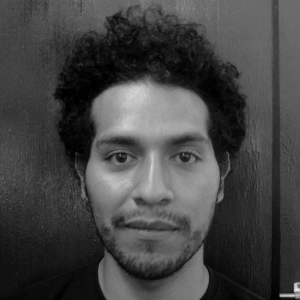
\includegraphics[scale=0.3]{jacobian.jpg}
\end{figure}
\textbf{Univ. Carlos Eduardo Caballero Burgoa}\\
Estudiante de Ing. de Sistemas en la Universidad Mayor de San Simón, Miembro de la sociedad cientifica
de Informática y Sistemas y Administrador del Laboratorio de Desarrollo del Departamento de
Informática y Sistemas. 

\end{document}